% --------------------------------------------------------------
% This is all preamble stuff that you don't have to worry about.
% Head down to where it says "Start here"
% --------------------------------------------------------------
 
\documentclass[12pt]{article}
 
\usepackage[margin=1in]{geometry} 
\usepackage{amsmath,amsthm,amssymb}
\usepackage[margin=1in]{geometry} 
\usepackage{amsmath,amsthm,amssymb}
%\usepackage[english}{babel} %Castellanización
\usepackage[T1]{fontenc} %escribe lo del teclado
\usepackage[utf8]{inputenc} %Reconoce algunos símbolos
\usepackage{lmodern} %optimiza algunas fuentes
\usepackage{graphicx}
\graphicspath{ {images/} }
\usepackage{hyperref} % Uso de links
\usepackage{caption}
\usepackage{subcaption}
 
\newcommand{\N}{\mathbb{N}}
\newcommand{\Z}{\mathbb{Z}}
 
\newenvironment{theorem}[2][Theorem]{\begin{trivlist}
\item[\hskip \labelsep {\bfseries #1}\hskip \labelsep {\bfseries #2.}]}{\end{trivlist}}
\newenvironment{lemma}[2][Lemma]{\begin{trivlist}
\item[\hskip \labelsep {\bfseries #1}\hskip \labelsep {\bfseries #2.}]}{\end{trivlist}}
\newenvironment{exercise}[2][Exercise]{\begin{trivlist}
\item[\hskip \labelsep {\bfseries #1}\hskip \labelsep {\bfseries #2.}]}{\end{trivlist}}
\newenvironment{problem}[2][Problem]{\begin{trivlist}
\item[\hskip \labelsep {\bfseries #1}\hskip \labelsep {\bfseries #2.}]}{\end{trivlist}}
\newenvironment{question}[2][Question]{\begin{trivlist}
\item[\hskip \labelsep {\bfseries #1}\hskip \labelsep {\bfseries #2.}]}{\end{trivlist}}
\newenvironment{corollary}[2][Corollary]{\begin{trivlist}
\item[\hskip \labelsep {\bfseries #1}\hskip \labelsep {\bfseries #2.}]}{\end{trivlist}}

\newenvironment{solution}{\begin{proof}[Solution]}{\end{proof}}
 
\begin{document}
 
% --------------------------------------------------------------
%                         Start here
% --------------------------------------------------------------
 
\title{DIABETES PREDICTION USING PIMA DIABETES DATASET}
\author{Vipin Rai P, Harshabh Mahant, Saurabh Singh\\
}

\maketitle
\section{Data Overview}
\begin{enumerate}
\item \textbf{Number of data points} : 768
\item \textbf{Number of features} : 8
\item \textbf{Features} :

Pregnancies : Number of times pregnant

Glucose : Plasma glucose concentration (2 hours in an oral glucose tolerance test)

BloodPressure : Diastolic blood pressure (mm Hg)

SkinThickness : Triceps skin fold thickness (mm)

Insulin : 2-Hour serum insulin (mu U/ml)

BMI : Body mass index

DiabetesPedigreeFunction - Diabetes pedigree function

Age : Age in years

\item \textbf{Number of classes} : 2

class '1' = Patient tested positive for diabetes

class '0' = Patient tested negative for diabetes \\

\item \textbf{Data points per class} :

class '1' : 268

class '0' : 500

\end{enumerate}

\begin{figure}[h]
\centering
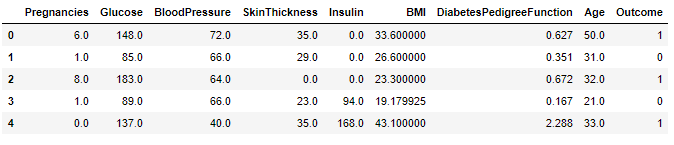
\includegraphics[scale=0.65]{df_head.PNG} 
\caption{Snapshot of dataset}
\label{etiqueta}
\end{figure}


\section{Data Preprocessing}

\subsection{Handling missing values}

\subsubsection{Observations:}
\begin{enumerate}
\item Columns containing missing data points cannot be filled with mean values as columns contains values corresponding to different patients. It is absurd to infer the missing data of a patient from distribution of data belonging to other patients.
\item Since the number of datapoints with missing values are less so we can replace the rows with missing values by 0 
\end{enumerate}
\begin{table}[h]
\begin{center}
\begin{tabular}{|c|c|c|c|}
\hline
 \textbf{Feature} & \textbf{Number of missing values(nan)}\\\hline
Pregnancies  & 26\\\hline
Glucose Value  & 16\\\hline
BloodPressure  & 0\\\hline
Skin Thickness & 22\\\hline
Insulin  & 0\\\hline
BMI  & 11\\\hline
Diabetes Pedigree Function  & 0\\\hline
Age  & 19\\\hline
\end{tabular}
\end{center}
\caption{Count of missing values}
\end{table}

\subsubsection{Inference}
\begin{enumerate}
\item Features SkinThickness and Insulin contains large number of zero values. Hence these two features can be ignored.
\item Columns Glucose,BloodPressure,BMI,Age will be greater than zero for a patient. Thus rows containing zero value for those features can be eliminated.
\item Pregnancies feature can contain zero values and such rows are retained.
\item In the next step rows containing negative values for features Pregancies,Glucose,BloodPressure, BMI, Age are eliminated. Negative value for those parameters are not valid
\item Rows containing zero values for features Glucose,BloodPressure,BMI,
Age are eliminated.
\end{enumerate}

\begin{table}[h]
\begin{center}
\begin{tabular}{|c|c|c|c|}
\hline
 \textbf{Feature} & \textbf{Number of zero values}\\\hline
Pregnancies  & 132\\\hline
Glucose Value  & 21\\\hline
BloodPressure  & 32\\\hline
Skin Thickness & 237\\\hline
Insulin  & 374\\\hline
BMI  & 21\\\hline
Diabetes Pedigree Function  & 0\\\hline
Age  & 19\\\hline
\end{tabular}
\end{center}
\caption{Count of zero values after replacing missing values with zeros}
\end{table}

\section{Exploratory Data Analysis}

\subsection{Probability Density Function}

\subsubsection{Observation}

\begin{enumerate}
\item It can be inferred that patients tested positive for diabetes had higher level of glucose. Most of them had values greater than 130.
\item BloodPressure values of both the classes patient overlap highly, so it won't be a major feature for classification.
\item Among patient tested positive for diabetes most of them had number of pergnancies greater than 3.
\item Most of the patients with diabetes had BMI value greater than 30.
\item Among patient tested negative most of them had diabetes pedigree function value less than 0.5 and if it is greater than 0.5 chances of having diabetes is more.
\item Count of patients with diabetes was higher for age group greater than 30.
\end{enumerate}

\begin{figure}
\centering
\begin{subfigure}{0.6\textwidth}
  \centering
  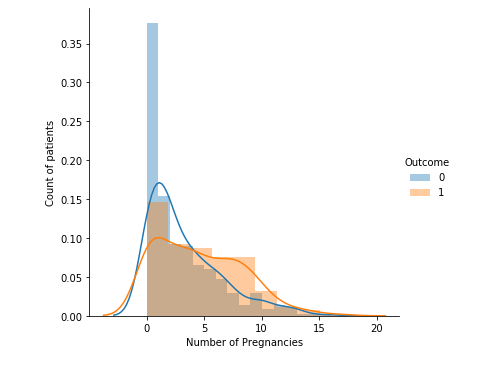
\includegraphics[width=1\linewidth]{preg.PNG}
  \label{fig:sub1}
\end{subfigure}%
\begin{subfigure}{.6\textwidth}
  \centering
  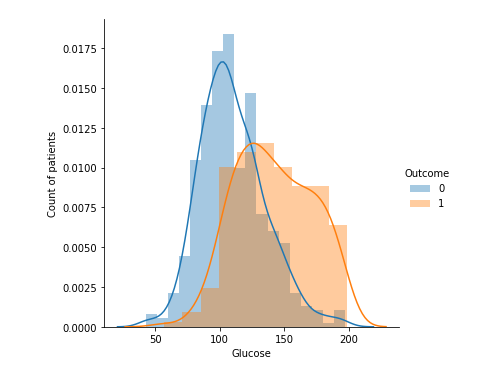
\includegraphics[width=1\linewidth]{glucose.PNG}
  \label{fig:sub2}
\end{subfigure}
\label{fig:test}
\end{figure}

\begin{figure}
\centering
\begin{subfigure}{0.6\textwidth}
  \centering
  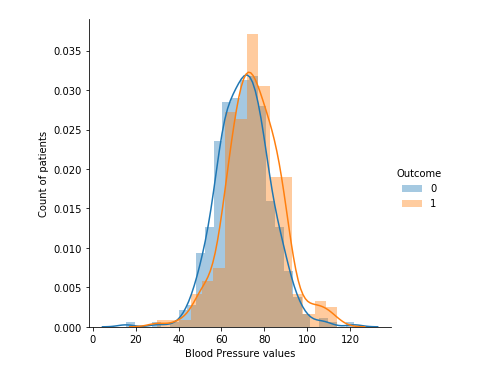
\includegraphics[width=1\linewidth]{BP.PNG}
  \label{fig:sub1}
\end{subfigure}%
\begin{subfigure}{.6\textwidth}
  \centering
  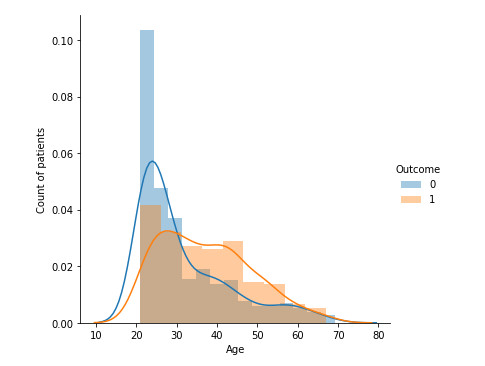
\includegraphics[width=1\linewidth]{age.PNG}
  \label{fig:sub2}
\end{subfigure}
\label{fig:test}
\end{figure}

\begin{figure}
\centering
\begin{subfigure}{0.6\textwidth}
  \centering
  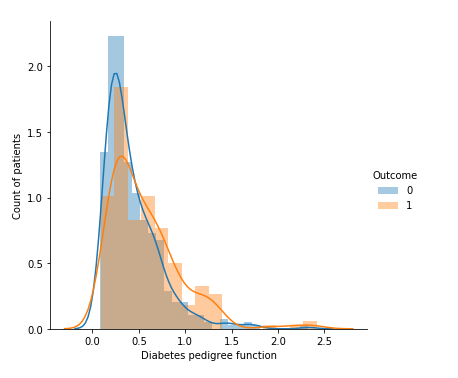
\includegraphics[width=1\linewidth]{dpfunct.PNG}
  \label{fig:sub1}
\end{subfigure}%
\begin{subfigure}{.6\textwidth}
  \centering
  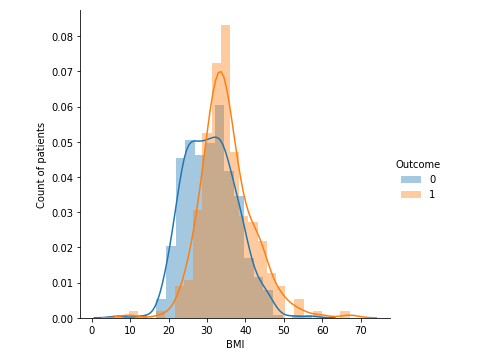
\includegraphics[width=1\linewidth]{BMI.PNG}
  \label{fig:sub2}
\end{subfigure}
\label{fig:test}
\end{figure}

\newpage
\subsection{Box Plots}

\begin{enumerate}
\item Box plot can be used to get more insight about the spread of data.
\item It will show the 50th , 25th and 75th percentiles vlaues of a particular feature. The length of the box will give the interquartile range (75th - 25th percentile) 
\end{enumerate}

\subsubsection{Pregnancies}

\begin{enumerate}
\item More than 50 percent of the patients tested positive for diabetes had atleast 3 pregnancies
\item 50 percent of patient tested negative had less than 2 pregnancies
\item It can be inferred that patient with more number of pregancies have higher chances of having diabetes
\end{enumerate}

\begin{figure}[h]
\centering
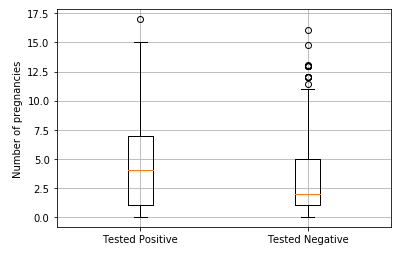
\includegraphics[scale=0.6]{boxplot_preg.PNG} 
\caption{Boxplot for Pregnancies}
\label{etiqueta}
\end{figure}

\subsubsection{BMI}

\begin{enumerate}
\item More than 75 percent of patients with diabetes had BMI greater than 30
\item 50 percent of patients without diabetes had BMI less than 30
\item BMI can be a major feature to decide whethere a patient is diabetic
\item Patient with BMI greater than 30 has higher chances of having diabetes
\end{enumerate}

\begin{figure}[h]
\centering
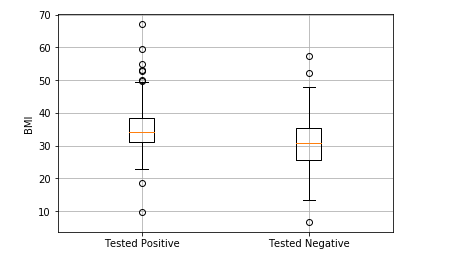
\includegraphics[scale=0.65]{boxplot_BMI.PNG} 
\caption{Boxplot for BMI}
\label{etiqueta}
\end{figure}

\subsubsection{Glucose}

\begin{enumerate}
\item More than 70 percent of patients with diabetes had glucode level higher than 120
\item Among patients tested negative 70 percent of them had glucose level less than 120
\item It is highly likely that patient has diabetes if his glucose level is more than 120
\end{enumerate}

\begin{figure}[h]
\centering
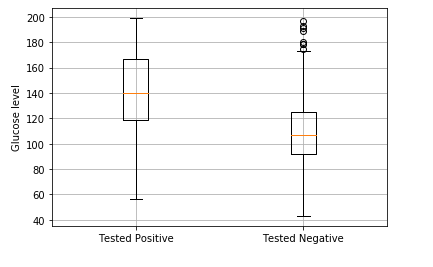
\includegraphics[scale=0.65]{boxplot_glucose.PNG} 
\caption{Boxplot for Glucose}
\label{etiqueta}
\end{figure}

\subsubsection{Blood Pressure}

\begin{enumerate}
\item Among of the patient tested negative for diabetes more than 75 percent of them had blood pressure in the range of 60 to 80 mm Hg
\item More than 50 percent of patients with diabetes had blood pressure higher than 70 mm Hg
\item Blood Pressure ranges are mostly overlaping for both classes of patients , however patient with blood pressure greater than 80 mm Hg is likely to have diabetes
\end{enumerate}

\begin{figure}[h]
\centering
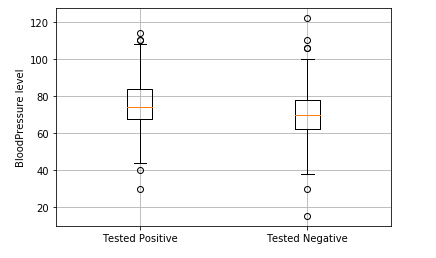
\includegraphics[scale=0.65]{boxplot_BP.PNG} 
\caption{Boxplot for Blood Pressure}
\label{etiqueta}
\end{figure}

\subsubsection{Age}

\begin{enumerate}
\item More than 75 percent of patients tested negative had age less than 38
\item More than 50 percent of patients with diabetes were of age greater than 35
\item Patient with age greater than 35 years have chances of having diabetes
\item Age can be considered as one of the major feature for classification
\end{enumerate}

\begin{figure}[h]
\centering
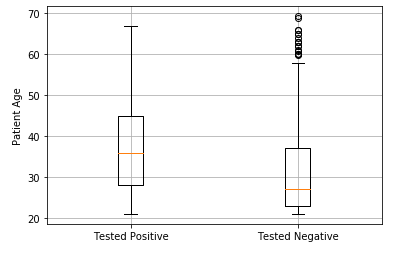
\includegraphics[scale=0.7]{boxplot_age.PNG} 
\caption{Boxplot for Age}
\label{etiqueta}
\end{figure}

\subsubsection{Diabetes Pedigree Function}

\begin{enumerate}
\item More than 50 percent of patient with Pedigree function value greater than 0.4 had diabetes
\item Among the patients tested negative for diabetes 50 percent of them had diabetes pedigree function vaue less than 0.3
\item If the diabetes pedigree function value is greater than 0.5 it is highly likely to have diabetes
\end{enumerate}

\begin{figure}[h]
\centering
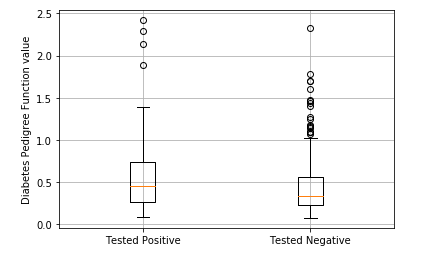
\includegraphics[scale=0.7]{boxplot_func.PNG} 
\caption{Boxplot for Diabetes Pedigree Function}
\label{etiqueta}
\end{figure}


\section{Model Building}


\begin{enumerate}
\item Features taken into cosideration    ["Pregnancies","Glucose","BloodPressure", "BMI", "Diabetes Pedigree Function", "Age"]
\item Since it's a classification problem logistic regression and knn algorithms are used to train the model.
\end{enumerate}

\subsection{Dimensionality Reduction using PCA}
\begin{enumerate}
\item PCA can be used to reduce the dimension from 6 features to 2 main features. Accuracy of model will be evaluated with and without dimensionality reduction.
\end{enumerate}

\newpage

\begin{figure}[h]
\centering
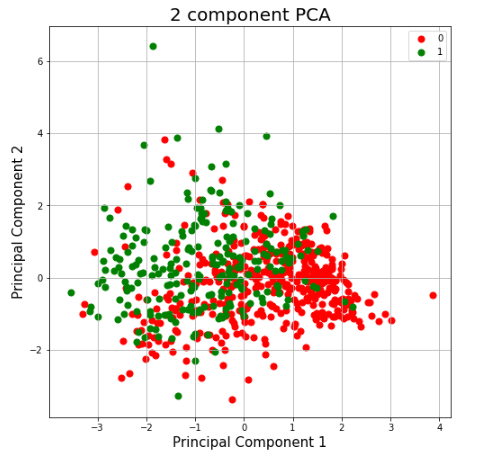
\includegraphics[scale=0.7]{PCA.PNG} 
\label{etiqueta}
\end{figure}


\begin{figure}[h]
\centering
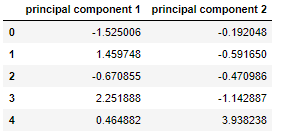
\includegraphics[scale=1]{PCA_table.PNG} 
\label{etiqueta}
\end{figure}


\subsection{Spliting dataset into train and test}

\begin{enumerate}
\item The given data is split into train and test in the ratio 8:2. 

\end{enumerate}

\subsection{Using Logistic Regression}

\subsubsection{Logistic regression without dimensionality reduction(without PCA)}
\begin{enumerate}
\item Accuracy of Logistic Regression without pca :  80.14705882352942
 

\end{enumerate}

\begin{table}[h]
\begin{center}
\begin{tabular}{|c|c|c|c|}
\hline
 \textbf{} & {Class 0} & {Class 1}\\\hline
Class 0  & 86 & 4\\\hline
Class 1  & 23 & 23\\\hline
\end{tabular}
\end{center}
\caption{Confusion matrix}
\end{table}

\subsubsection{Logistic regression with dimensionality reduction(PCA)}
\begin{enumerate}
\item Accuracy of Logistic Regression with pca :  75.0

\end{enumerate}

\begin{table}[h]
\begin{center}
\begin{tabular}{|c|c|c|c|}
\hline
 \textbf{} & {Class 0} & {Class 1}\\\hline
Class 0  & 86 & 4\\\hline
Class 1  & 30 & 16\\\hline
\end{tabular}
\end{center}
\caption{Confusion matrix}
\end{table}

\subsection{Using K-Nearest Neighbour}


\begin{enumerate}
\item From the scatter plot(Principal component 1 vs principal component 2) it can be inferred that two classes are not linearly separable.
\item Logistic regression might be failing to fit a accurate plane that can separate the two classes with more accuracy.
\item K-NN algorithm finds k-nearest neigbours for a data point and decides it's class based on majotity rule. 
\item Best values of k can be chosen by a technique called cross validation (10 fold). Here the train data is split into 10 parts. In each interval one part among 10 is chosen as test and knn is applied on that. Mean of accuracy is calculated for all 10 parts(cv scores). This is repeated for different values of k. k value that gives best accuracy is chosen as optimal k value.
\item Model is designed for dataset with and without pca and accuracy is tested for both cases.
\end{enumerate}


\subsubsection{K-NN without dimensionality reduction(without PCA)}

\begin{enumerate}
\item The optimal value of k(neighbours) = 33.
\item Accuracy of knn without pca : 83.088235

\end{enumerate}

\begin{table}[h]
\begin{center}
\begin{tabular}{|c|c|c|c|}
\hline
 \textbf{} & {Class 0} & {Class 1}\\\hline
Class 0  & 88 & 2\\\hline
Class 1  & 21 & 25\\\hline
\end{tabular}
\end{center}
\caption{Confusion matrix}
\end{table}

\subsubsection{K-NN with dimensionality reduction(PCA)}
\begin{enumerate}
\item The optimal value of k(neighbours) = 41.
\item Accuracy of knn with pca : 75.73529411764706
\end{enumerate}

\begin{table}[h]
\begin{center}
\begin{tabular}{|c|c|c|c|}
\hline
 \textbf{} & {Class 0} & {Class 1}\\\hline
Class 0  & 86 & 4\\\hline
Class 1  &29 & 17\\\hline
\end{tabular}
\end{center}
\caption{Confusion matrix}
\end{table}

\section{Conclusion}

\begin{enumerate}
\item Data preprocessing was done to replace the missing values with appropriate ones. The rows containing invalid inputs(like zero values) for certain columns were eliminated.
\item Exploratoty data analysis was made to get insight about the distribution of the data with respect to different  features. Probability density function and Box plot tools were used for analysis.
\item PCA was used for dimensionality reduction and principal components were plotted using 2d-scatter plot. 
\item Model was trained using Logistic regression. Model was trained with and without dimensionality reduction.Accuracy was ranging between 75 to 80 percent.
\item Model was trained using K-NN. Optimal value for k was chosen using cross validation technique. Model was trained with and without dimensionality reduction.Accuracy was ranging between 75 to 80 percent.

\end{enumerate}















% --------------------------------------------------------------
%     You don't have to mess with anything below this line.
% --------------------------------------------------------------
 
\end{document}